\documentclass[12pt]{article}

\usepackage{amsmath,amsthm,amsfonts,amssymb,amsxtra}
\usepackage{tikz,array}
\usetikzlibrary{arrows}
\renewcommand{\theenumi}{(\alph{enumi})} 
\renewcommand{\labelenumi}{\theenumi}

\pagestyle{empty}
\setlength{\textwidth}{7in}
\setlength{\oddsidemargin}{-0.5in}
\setlength{\topmargin}{-1.0in}
\setlength{\textheight}{9.5in}

\theoremstyle{definition}
\newtheorem{problem}{Problem}

\begin{document}

\noindent{\large\bf MATH 242}\hfill{\large\bf Final Exam}\hfill{\large\bf
Summer 2017}\hfill{\large\bf Page 1/10}\hrule

\bigskip
\begin{center}
\begin{tabular}{|ll|}
\hline & \cr
{\bf Name: } & \makebox[12cm]{\hrulefill}\cr & \cr
{\bf VIP ID:} & \makebox[12cm]{\hrulefill}\cr & \cr
\hline
\end{tabular}
\end{center}
\begin{itemize}
  \item Write your name and your VIP ID in the space provided above.
  \item The test has ten (10) pages, including this one and two pages of scratch paper at the end.  One of those pages contains a \emph{Laplace table}.  Do \textbf{NOT} detach those pages.
  \item You have 150 minutes (2.5 hours) to complete the exam.
  \item Show sufficient work to justify all answers unless otherwise stated in the problem.  Correct answers with inconsistent work may not be given credit.
  \item Credit for each problem is given at the right of each problem number.
  \item You must show proficiency solving theoretical questions on differential equations.  If the combined score of pages 2,3,4 is not at least 30 points, none of the application problems in pages 5,6,7,8 will be graded.
\end{itemize}
\hrule

\begin{center}
\begin{tikzpicture}
\draw (0,0) node[scale=0.8]{%
\begin{tabular}{|c|c|c|}
\hline
&&\cr
{\large\bf Page} & {\large\bf Max} & {\large\bf Points} \cr
&&\cr
\hline
&&\cr
{\Large } & \Large  & \cr
&&\cr
\hline
&&\cr
{\Large 2} & \Large 20 & \cr
&&\cr
\hline
&&\cr
{\Large 3} & \Large 20 & \cr
&&\cr
\hline
&&\cr
{\Large 4} & \Large 20 & \cr
&&\cr
\hline\hline
&&\cr
{\large\bf Total} & \Large 60 & \cr
&&\cr
\hline
\end{tabular} \begin{tabular}{|c|c|c|}
\hline
&&\cr
{\large\bf Page} & {\large\bf Max} & {\large\bf Points} \cr
&&\cr
\hline
&&\cr
{\Large 5} & \Large 10 & \cr
&&\cr
\hline
&&\cr
{\Large 6} & \Large 10 & \cr
&&\cr
\hline
&&\cr
{\Large 7} & \Large 10 & \cr
&&\cr
\hline
&&\cr
{\Large 8} & \Large 10 & \cr
&&\cr
\hline\hline
&&\cr
{\large\bf Total} & \Large 40 & \cr
&&\cr
\hline
\end{tabular}};
\end{tikzpicture}
\end{center}
\hrule

\vspace{0.6cm}

\begin{quotation}
\noindent I, \makebox[8cm]{\hrulefill}, have chosen to take the final exam for Section 202 of Math 242 in the Summer'17 session.  The grade I earn on this final exam will be my grade for the course and once I begin this exam, I must complete it.  I am hereby declining my option to take the grade I currently have in the course, and I realize that my final course grade, as determined by this final exam alone, may be lower than my current grade.  I realize this decision is final.

\vspace{1cm}

\noindent Student Signature: \makebox[8cm]{\hrulefill} Date: \makebox[3cm]{\hrulefill}


\end{quotation}
\newpage

%%%%%%%%%%%%%%%%%%%%%%%%%%%%%%%%%%%%% Page 2
\noindent{\large\bf MATH 242}\hfill{\large\bf Final Exam}\hfill{\large\bf Summer 2017}\hfill{\large\bf Page 2/10}\hrule

\bigskip
\begin{problem}[20 pts---5 pts each part]
Consider the following differential equation: 
\begin{equation*}
y' = x(y^2+2y-8)
\end{equation*}
\begin{enumerate}
  \item Which of the following is its slope field?
  \begin{flushleft}
  \begin{tabular}{ccc}
  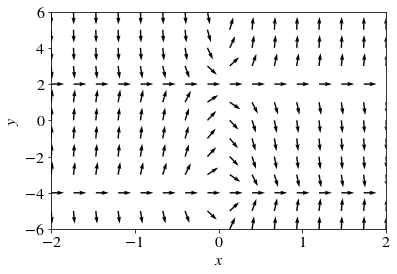
\includegraphics[width=0.33\linewidth]{fquiver1.png} &
  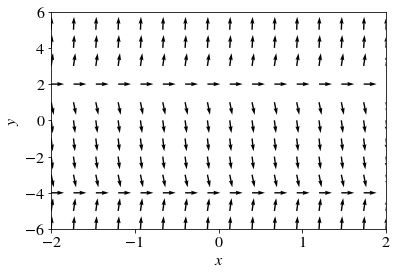
\includegraphics[width=0.33\linewidth]{fquiver2.png} &
  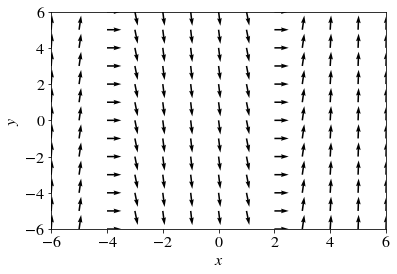
\includegraphics[width=0.33\linewidth]{fquiver3.png}
  \end{tabular}
  \end{flushleft}
  \item Employ Euler's method with a time step $h=0.5$ to approximate numerically the solution to the \emph{initial value problem} $y'=x(y^2+2y-8)$ with initial condition $y(0)=0$.
  \begin{flushright}
  \begin{tikzpicture}
  \draw (0,0) node [scale=0.73]{%
  \begin{tabular}{|c||c|c|c|}
  \hline
  $n$ & $x_n$ & $y_n$ & $f(x_n, y_n)$ \\ 
  \hline \hline
  &&& \\
  $0$ & \hspace{1cm} & \hspace{1.25cm} & \hspace{3cm} \\
  &&& \\ \hline
  &&& \\
  $1$ &&& \\
  &&& \\ \hline
  &&& \\
  $2$ &&& \\
  &&& \\ \hline
  \end{tabular}
  };
  \end{tikzpicture}
  \end{flushright}
  \item Find an \emph{implicit solution} to the initial value problem $y'=x(y^2+2y-8), y(0)=0$.
  \vspace{5.5cm}
  \begin{flushright}
  \begin{tikzpicture}
  \draw (-1cm, 0.5cm) node{Solution:};
  \draw (0cm,-0.2cm) rectangle (8cm,1.2cm);
  \end{tikzpicture}
  \end{flushright}
  \item Find an \emph{explicit solution} to the initial value problem $y'=x(y^2+2y-8), y(0)=2$
  \begin{flushright}
  \begin{tikzpicture}
  \draw (-0.7cm, 0.5cm) node{$y(x)=$};
  \draw (0cm,-0.2cm) rectangle (8cm,1.2cm);
  \end{tikzpicture}
  \end{flushright}
\end{enumerate}
\end{problem} 

\newpage

%%%%%%%%%%%%%%%%%%%%%%%%%%%%%%%%%%%%% Page 3
\noindent{\large\bf MATH 242}\hfill{\large\bf Final Exam}\hfill{\large\bf
Summer 2017}\hfill{\large\bf Page 3/10}\hrule

\bigskip
\begin{problem}[20 pts---10 pts each part]
Solve the following linear differential equations.  \newline Do \textbf{NOT} employ any Laplace Transform techniques.
\begin{enumerate}
  \item $y'+ \dfrac{2}{x} y = x-1$
  \vspace{7cm}
  \begin{flushright}
  \begin{tikzpicture}
  \draw (-0.7cm, 0.5cm) node{$y(x)=$};
  \draw (0cm,-0.2cm) rectangle (7cm,1.2cm);
  \end{tikzpicture}
  \end{flushright}
  \item $y''+3y'+2y=x-2$
  \vspace{9.5cm}
  \begin{flushright}
  \begin{tikzpicture}
  \draw (-0.7cm, 0.5cm) node{$y(x)=$};
  \draw (0cm,-0.2cm) rectangle (7cm,1.2cm);
  \end{tikzpicture}
  \end{flushright}
\end{enumerate}
\end{problem} 

\newpage

%%%%%%%%%%%%%%%%%%%%%%%%%%%%%%%%%%%%% Page 4
\noindent{\large\bf MATH 242}\hfill{\large\bf Final Exam}\hfill{\large\bf
Summer 2017}\hfill{\large\bf Page 4/10}\hrule

\bigskip
\begin{problem}[10 pts]
Use techniques based on the Laplace transform to solve the initial value problem $y''+3y'+2y=x$ that satisfies $y(0)=0, y'(0)=2$.
\vspace{8cm}
\begin{flushright}
\begin{tikzpicture}
\draw (0cm,-0.2cm) rectangle (5cm,1.2cm);
\end{tikzpicture}
\end{flushright}
\end{problem}
\hrule

\begin{problem}[5 pts]
Find the Laplace transform of $f(x) = 12x e^{-3x} \sin(5x)$
\vspace{5cm}

\begin{flushright}
\begin{tikzpicture}
\draw (-0.75cm, 0.5cm) node{$F(s) =$};
\draw (0cm,-0.2cm) rectangle (5cm,1.2cm);
\draw (4cm, 0cm) node {$(s> \quad)$};
\end{tikzpicture}
\end{flushright}
\end{problem}
\hrule

\begin{problem}[5 pts]
Find the inverse Laplace transform of $F(s) =\dfrac{s-3}{(s-3)^2+16}$ for $s>3$.
\vspace{2cm}
\begin{flushright}
\begin{tikzpicture}
\draw (-0.75cm, 0.5cm) node{$f(x) =$};
\draw (0cm,-0.2cm) rectangle (5cm,1.2cm);
\end{tikzpicture}
\end{flushright} 

\end{problem}
\newpage

%%%%%%%%%%%%%%%%%%%%%%%%%%%%%%%%%%%%% Page 5
\noindent{\large\bf MATH 242}\hfill{\large\bf Final Exam}\hfill{\large\bf
Summer 2017}\hfill{\large\bf Page 5/10}\hrule

\bigskip
\begin{problem}[10 pts]
Consider a bolt shot straight upward with initial velocity $v_0=49~\mathrm{m}/\mathrm{s}$ from a crossbow at ground level.  Assume air resistance proportional to the square of the velocity, with $\rho = 0.0011$.  Compute the maximum height of the bolt, and the time it takes it to reach that point.
\vspace{19cm}
\begin{flushright}
\begin{tikzpicture}
\draw (-1.25cm, 0.5cm) node{Max.~height:};
\draw (0cm,-0.2cm) rectangle (5cm,1.2cm);
\begin{scope}[xshift=9cm]
\draw (-1.25cm, 0.5cm) node{Time aloft:};
\draw (0cm,-0.2cm) rectangle (5cm,1.2cm);
\end{scope}
\end{tikzpicture}
\end{flushright}
\end{problem}
\newpage

%%%%%%%%%%%%%%%%%%%%%%%%%%%%%%%%%%%%% Page 6
\noindent{\large\bf MATH 242}\hfill{\large\bf Final Exam}\hfill{\large\bf
Summer 2017}\hfill{\large\bf Page 6/10}\hrule

\bigskip
\begin{problem}[10 pts]
Suppose that at time $t = 0$, ten thousand people in a city with population $M = 100$ thousand people have heard a certain rumor. After one week the number $P(t)$ of those who have heard it has increased to twenty thousand. Assuming that $P(t)$ satisfies a logistic equation, when will 80\% of the city's population have heard the rumor?
\vspace{19.5cm}
\begin{flushright}
\begin{tikzpicture}
\draw (-0.5cm, 0.5cm) node{$t=$};
\draw (0cm,-0.2cm) rectangle (5cm,1.2cm);
\end{tikzpicture}
\end{flushright}
\end{problem}
\newpage

%%%%%%%%%%%%%%%%%%%%%%%%%%%%%%%%%%%%% Page 7
\noindent{\large\bf MATH 242}\hfill{\large\bf Final Exam}\hfill{\large\bf
Summer 2017}\hfill{\large\bf Page 7/10}\hrule

\bigskip
\begin{problem}[10 pts---5 pts each]
Suppose that a mass in a mass-spring-dashpot system with $m=25$, $c=10$, and $k=226$ is set in motion with $x(0)=20$ and $x'(0)=41$. 
\begin{enumerate}
  \item Find the position function $x(t)$ and produce a rough sketch of the solution.  Is this a critically damped, over-damped or under-damped motion?
  \vspace{4cm}
  \begin{flushright}
  \begin{tikzpicture}
  \draw (-0.7cm, 0.5cm) node{$x(t)=$};
  \draw (0cm,-0.2cm) rectangle (6cm,1.2cm);
  \end{tikzpicture}
  \end{flushright}
  \item Find the pseudoperiod of the oscillations and the amplitude (also known as \emph{envelope curves})
  \vspace{12cm}
  \begin{flushright}
  \begin{tikzpicture}
  \draw (-1.35cm, 0.5cm) node{Pseudoperiod:};
  \draw (0cm,-0.2cm) rectangle (3cm,1.2cm);
  \begin{scope}[xshift=8cm]
  \draw (-1.7cm, 0.5cm) node{Envelope Curves:};
  \draw (0cm,-0.2cm) rectangle (3cm,1.2cm);
  \end{scope}
  \end{tikzpicture}
  \end{flushright}
\end{enumerate}
\end{problem}
\newpage

%%%%%%%%%%%%%%%%%%%%%%%%%%%%%%%%%%%%% Page 8
\noindent{\large\bf MATH 242}\hfill{\large\bf Final Exam}\hfill{\large\bf
Summer 2017}\hfill{\large\bf Page 8/10}\hrule

\bigskip
\begin{problem}[10 pts]
A water tank has the shape obtained by revolving the curve $y=x^{4/3}$ around the $y$--axis.  A plug at the bottom is removed at 12 noon, when the depth of the water in the tank is 12~ft.  At 1 pm the depth of the water is 6~ft.  When will the tank be empty?
\vspace{19cm}
\begin{flushright}
\begin{tikzpicture}
\draw (-0.5cm, 0.5cm) node{$t=$};
\draw (0cm,-0.2cm) rectangle (3cm,1.2cm);
\end{tikzpicture}
\end{flushright}
\end{problem}
\newpage

%%%%%%%%%%%%%%%%%%%%%%%%%%%%%%%%%%%%% Page 9
\noindent{\large\bf MATH 242}\hfill{\large\bf Final Exam}\hfill{\large\bf
Summer 2017}\hfill{\large\bf Page 9/10}\hrule

\bigskip
\begin{center}
%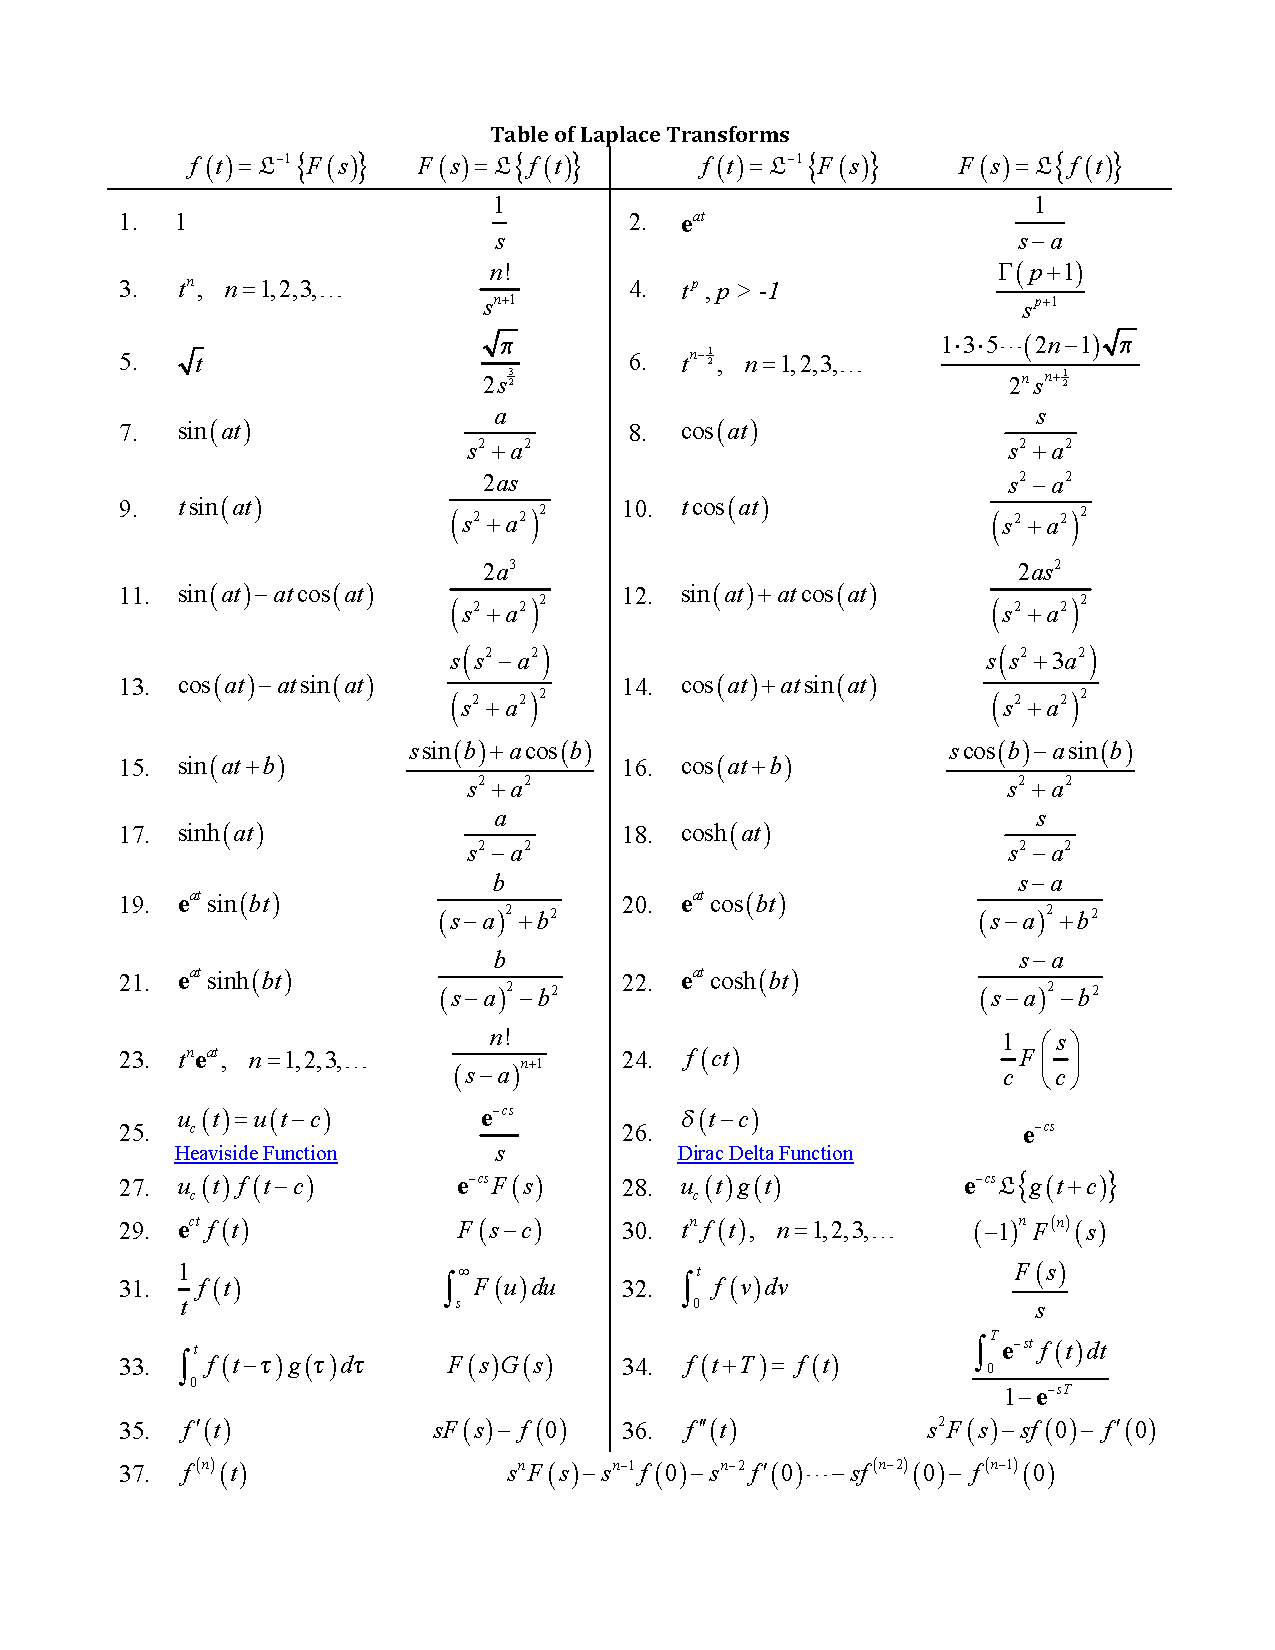
\includegraphics[width=\linewidth]{table.pdf}
\begin{tikzpicture}
\node[scale=0.97]{
\begin{tabular}{|m{1.2cm}|m{4.3cm}l||m{2.1cm}|m{4.3cm}l|}
\hline
$f(x)$\raisebox{0.5cm} & $\mathcal{L}\{f\}=\int_0^\infty e^{-sx}f(x)\, dx$\raisebox{0.5cm} & &
\raisebox{0.5cm} & \raisebox{0.5cm} & \\[0.4cm] 
\hline \hline
$1$ & $\dfrac{1}{s}$\raisebox{0.6cm} & $s>0$ &
$cf(x)\pm g(x)$ & $cF(s) \pm G(s)$\raisebox{0.4cm} & $s>max(a,b)$ \\[0.4cm]
\hline
$x^n$ & $\dfrac{n!}{s^{n+1}}$\raisebox{0.6cm} & $s>0$ & $e^{\alpha x}f(x)$ & $F(s-\alpha)$\raisebox{0.4cm} & $s>a+\alpha$ \\[0.4cm]
\hline
$x^p$ & $\frac{p}{s} \mathcal{L}\{ x^{p-1} \}$\raisebox{0.6cm} & $s>0$ &
$x^n f(x)$ & $(-1)^n F^{(n)}(s)$\raisebox{0.4cm} & $s>a$ \\[0.4cm]
\hline
$e^{\alpha x}$ & $\dfrac{1}{s-\alpha}$\raisebox{0.6cm} & $s>\alpha$ & $f'(x)$ & $s F(s) -f(0)$\raisebox{0.4cm} & $s>a$ \\[0.4cm]
\hline
$\sin \beta x$ & $\dfrac{\beta}{s^2+\beta^2}$\raisebox{0.6cm} & $s>0$  &\raisebox{0.4cm} & & \\[0.4cm]
\hline
$\cos \beta x$ & $\dfrac{s}{s^2+\beta^2}$\raisebox{0.6cm} & $s>0$ & \raisebox{0.4cm} & & \\[0.4cm]
\hline
\end{tabular} };
\end{tikzpicture}
\end{center}

\hrule

\bigskip
\noindent You may use this as scratch paper.

\newpage

%%%%%%%%%%%%%%%%%%%%%%%%%%%%%%%%%%%%% Page 10
\noindent{\large\bf MATH 242}\hfill{\large\bf Final Exam}\hfill{\large\bf
Summer 2017}\hfill{\large\bf Page 10/10}\hrule

\bigskip
\Large Scratch paper

\end{document}